\documentclass[10pt]{article}

\usepackage[margin=0.82in]{geometry}
\usepackage[T1]{fontenc}
\usepackage[utf8]{inputenc}
\usepackage{newtxtext,newtxmath}
\usepackage{microtype}
\usepackage{graphicx}
\usepackage{booktabs}
\usepackage{array}
\usepackage{amsmath}
\usepackage{pifont}
\usepackage{xcolor}
\usepackage{natbib}
\usepackage[hidelinks]{hyperref}
\usepackage[font=small,labelfont=bf]{caption}

\newcommand{\method}{SHARE-ViT}
\newcommand{\look}{\textsc{Look}}
\newcommand{\yes}{\ding{51}}
\newcommand{\no}{--}
\newcommand{\R}{\mathbb{R}}
\newcommand{\geom}[2]{\ensuremath{\mathcal{G}_{#1,#2}}}
\definecolor{thirdblue}{HTML}{2F6DB2}
\newcommand{\third}[1]{\textcolor{thirdblue}{#1}}
\newcommand{\figplaceholder}[2]{%
  \fbox{\parbox[c][#1][c]{0.94\linewidth}{\centering\bfseries #2}}}

\title{SHARE-ViT: Shared Hexagonal Angle--Scale Routing Enhancement\\
for Vision Transformers}
\author{Anonymous Authors}
\date{}

\begin{document}
\maketitle

\begin{abstract}
Vision Transformers typically begin with a square, axis-aligned patch
projection. This front end has no explicit representation of local pose or
scale, while absolute positional embeddings encode where a token is but not
which image-conditioned direction it should attend to. We introduce
\method{}, a geometric enhancement that couples a shared hexagonal angle--scale
tokenizer with pose-conditioned attention bias. Images are sampled on a
staggered hexagonal lattice, compared with learned variable-resolution polar
prototypes at two scales and several orientations, and projected into compact
cosine/sine pose coordinates. A null-softmax route allows a prototype to
abstain when no tested pose is suitable. The same geometric language drives two
directed attention mechanisms: Image \look{} estimates pose from the input
image, whereas Feature \look{} estimates it directly from the paired tokenizer
coordinates and can share one pose probe across several Transformer layers.
In controlled 20-epoch training from scratch on ImageNet-100, the
six-direction tokenizer with Image \look{} reaches 55.04\% top-1 and 81.80\%
top-5 accuracy, compared with 51.52\% and 79.12\% for a standard
DeiT-Tiny-sized baseline. Feature \look{} alone with PE reaches 55.18\% top-1;
combining both \look{} branches with a three-layer probe-sharing span reaches
55.54\% top-1 and 81.82\% top-5. These variants remain below the baseline
parameter count. The results support explicit local pose and scale as a useful
interface between image sampling and global attention, but do not establish
exact equivariance or broad cross-dataset superiority.
\end{abstract}

\section{Introduction}

Vision Transformers (ViTs) apply self-attention to a sequence of image tokens
\citep{dosovitskiy2021vit,touvron2021deit}. Their global interaction is
attractive, but the sequence is normally created by a square patch projection
with one learned weight for every Cartesian location. On a square lattice,
axial neighbors are one grid step away while diagonal neighbors are
$\sqrt{2}$ steps away. Equal changes in discrete direction therefore do not
correspond to equal spatial displacements. The tokenizer also entangles local
appearance with one canonical orientation and scale.

Recent tokenization studies make this front-end choice increasingly explicit.
FlexiViT interpolates patch-embedding parameters across patch sizes
\citep{beyer2023flexivit}, while MSViT selects mixed token scales according to
image content \citep{havtorn2023msvit}. These methods improve scale flexibility,
but they do not explicitly represent the orientation of a matched local
pattern.

Position encoding addresses a related but different issue. Absolute
embeddings tell the model where a token occurs, and relative position methods
tell attention how two token indices are displaced \citep{wu2021irpe}.
More recent work extends rotary embeddings to two-dimensional ViT coordinates
\citep{heo2024ropevit} and redesigns tokenization, attention, patch merging,
and positional encoding for exact circular shift equivariance
\citep{rojasgomez2024shiftequiv}.
Neither mechanism, by itself, asks whether the image evidence supports a
particular pose, nor does it convert that evidence into a directed search
pattern. Local-window Transformers such as Swin introduce efficient spatial
locality \citep{liu2021swin}, whereas conditional position encodings generate
input-dependent position signals \citep{chu2021cpvt}. Our goal is
complementary: construct an explicit local angle--scale representation before
global attention and reuse it to condition where each attention head looks.

Rotation-aware convolution has a long history. Group-equivariant networks
share filters under discrete transformations \citep{cohen2016gcnn}, active
rotating filters materialize oriented responses \citep{zhou2017orn}, and
harmonic networks encode rotations with circular harmonics
\citep{worrall2017harmonic}. Hexagonal convolution reduces lattice anisotropy
and permits additional rotational weight sharing \citep{hoogeboom2018hexaconv}.
Recent Transformer designs carry this program further through discrete
$E(2)$-equivariant attention \citep{xu2023e2vit}, continuous harmonic
representations \citep{karella2024harmformer}, and steerable Fourier features
\citep{kundu2025steerable}.
\method{} builds rotation-shared local matching on a Hex lattice and then
transfers the resulting pose evidence to Transformer attention. It is a
pose-aware enhancement of a ViT rather than a strict group-equivariant model.

Our contributions are:
\begin{itemize}
  \item a Hex-centered, multi-scale rotation-matching tokenizer: shared
  variable-resolution polar prototypes are evaluated over discrete poses, a
  null route suppresses unsupported matches, and circular moments preserve
  compact directional features on a common token graph;
  \item two pose-conditioned attention biases derived from the same geometric
  representation: Image \look{} reads direction and scale from raw-image
  patches, while Feature \look{} reads pose from tokenizer features and allows
  probe reuse across nearby Transformer layers. Thus local pose evidence is
  used both to construct tokens and to direct later global attention.
\end{itemize}

\begin{figure}[t]
  \centering
  \includegraphics[width=\textwidth]{figs/01_share_vit_full_architecture.pdf}
  \caption{Overview of \method{}. Hex Tokenization constructs the shared
  lattice, MAMS Projection extracts multi-scale multi-pose token features, and
  Image and Feature \look{} paths inject complementary directed attention
  biases across the Transformer backbone.}
  \label{fig:architecture}
\end{figure}

\section{Related Work}

\paragraph{Visual tokenization and spatial bias.}
ViT maps non-overlapping square patches to tokens and adds learned positional
embeddings \citep{dosovitskiy2021vit}. DeiT demonstrates effective training of
this architecture on ImageNet without external pretraining
\citep{touvron2021deit}. Later models inject more local structure: Swin
restricts attention to shifted windows \citep{liu2021swin}, iRPE introduces
directional relative position terms \citep{wu2021irpe}, and CPVT generates
conditional positional encodings from local neighborhoods
\citep{chu2021cpvt}. RoPE-ViT adapts rotary coordinates to two-dimensional
visual tokens and improves resolution extrapolation \citep{heo2024ropevit},
while recent shift-equivariant ViTs treat tokenization and positional encoding
as part of the equivariance problem \citep{rojasgomez2024shiftequiv}.
\method{} preserves global attention. Locality enters
through geometric token formation and an input-conditioned directed field,
rather than a fixed window or only an index-based lookup table.

\paragraph{Flexible visual tokenization.}
Patch size controls both the visual support of a token and the sequence length.
FlexiViT randomizes patch size and interpolates patch and position parameters so
one ViT can operate at several resolutions \citep{beyer2023flexivit}. MSViT
instead uses a learned gate to construct mixed-scale token sequences
\citep{havtorn2023msvit}. These approaches vary token scale or allocation;
our tokenizer keeps one shared Hex token graph and evaluates multiple support
scales and orientations at each center before projecting a token.

\paragraph{Rotation-aware representations.}
G-CNNs formalize weight sharing over transformation groups
\citep{cohen2016gcnn}. ORNs rotate active filters and retain orientation
channels \citep{zhou2017orn}, while harmonic networks use circular bases to
encode rotation \citep{worrall2017harmonic}. At the Transformer boundary,
Equi-ViT replaces patch embedding with radially symmetric Gaussian-mixture-ring
convolutions \citep{chen2026equivit}; GE-ViT instead lifts tokens to a joint
spatial--orientation domain and preserves a discrete group axis through
self-attention \citep{xu2023e2vit}; and Steerable Transformers carry Fourier
irreducible representations through attention, normalization, and feed-forward
layers \citep{kundu2025steerable}. Harmformer combines a harmonic convolutional
stem with attention to obtain continuous roto-translation equivariance
\citep{karella2024harmformer}. These methods motivate our shared prototypes
and cosine/sine pose coordinates, but our current tokenizer learns no A/B
orthogonal value basis: it directly takes a fixed first circular moment of the
routed pose scores. The present model samples a finite set of orientations and
does not enforce an equivariance identity; we therefore use \emph{pose-aware}
and \emph{rotation-shared}, rather than \emph{rotation-equivariant}, in our
claims.

\paragraph{Hexagonal image processing.}
Hexagonal lattices provide six equidistant first-ring neighbors. HexaConv shows
that hexagonal planar and group convolutions can reduce lattice anisotropy and
improve rotational parameter sharing \citep{hoogeboom2018hexaconv}. Our input
remains a conventional Cartesian image. We place patch centers on staggered
rows and sample circular supports by interpolation, requiring neither native
hexagonal camera data nor a hexagonal storage format.

\section{Method}

\subsection{Overview}

\method{} has a tokenizer and two optional directed-bias paths
(Fig.~\ref{fig:architecture}). The tokenizer maps an image to a sequence of
192-D tokens. Image \look{} independently re-samples the input image; Feature
\look{} instead interprets the token dimensions as geometric pairs. Both
produce pose probabilities that rotate learned radial--angular fields before
the fields are added to attention logits. The paths share a geometric
language---scale, direction, polar sampling, and null routing---but do not have
to share learned prototype parameters.

\subsection{Hexagonal patch centers}

Let $x\in\R^{H\times W\times3}$ be an input image. Patch centers are placed on
alternating horizontally shifted rows, producing a staggered Hex lattice. At
$224\times224$ resolution, the current geometry yields 195 image tokens,
close to the 196 tokens of a standard $14\times14$ DeiT tokenizer. Reflection
padding handles image boundaries. Two circular supports with diameters
$K\in\{24,12\}$ share every center, so scale comparison does not alter the
token graph.

Each support uses a cosine-shaped radial cover $c_K(u)$. We preserve its
accumulated response magnitude rather than normalizing it to unit mass. The
smaller support is compensated by
\begin{equation}
  \gamma_K=\frac{\sum_u c_{24}(u)}{\sum_u c_K(u)},
  \label{eq:cover}
\end{equation}
removing a response difference caused only by the number of covered pixels.

\begin{figure}[t]
  \centering
  \makebox[\textwidth][c]{%
    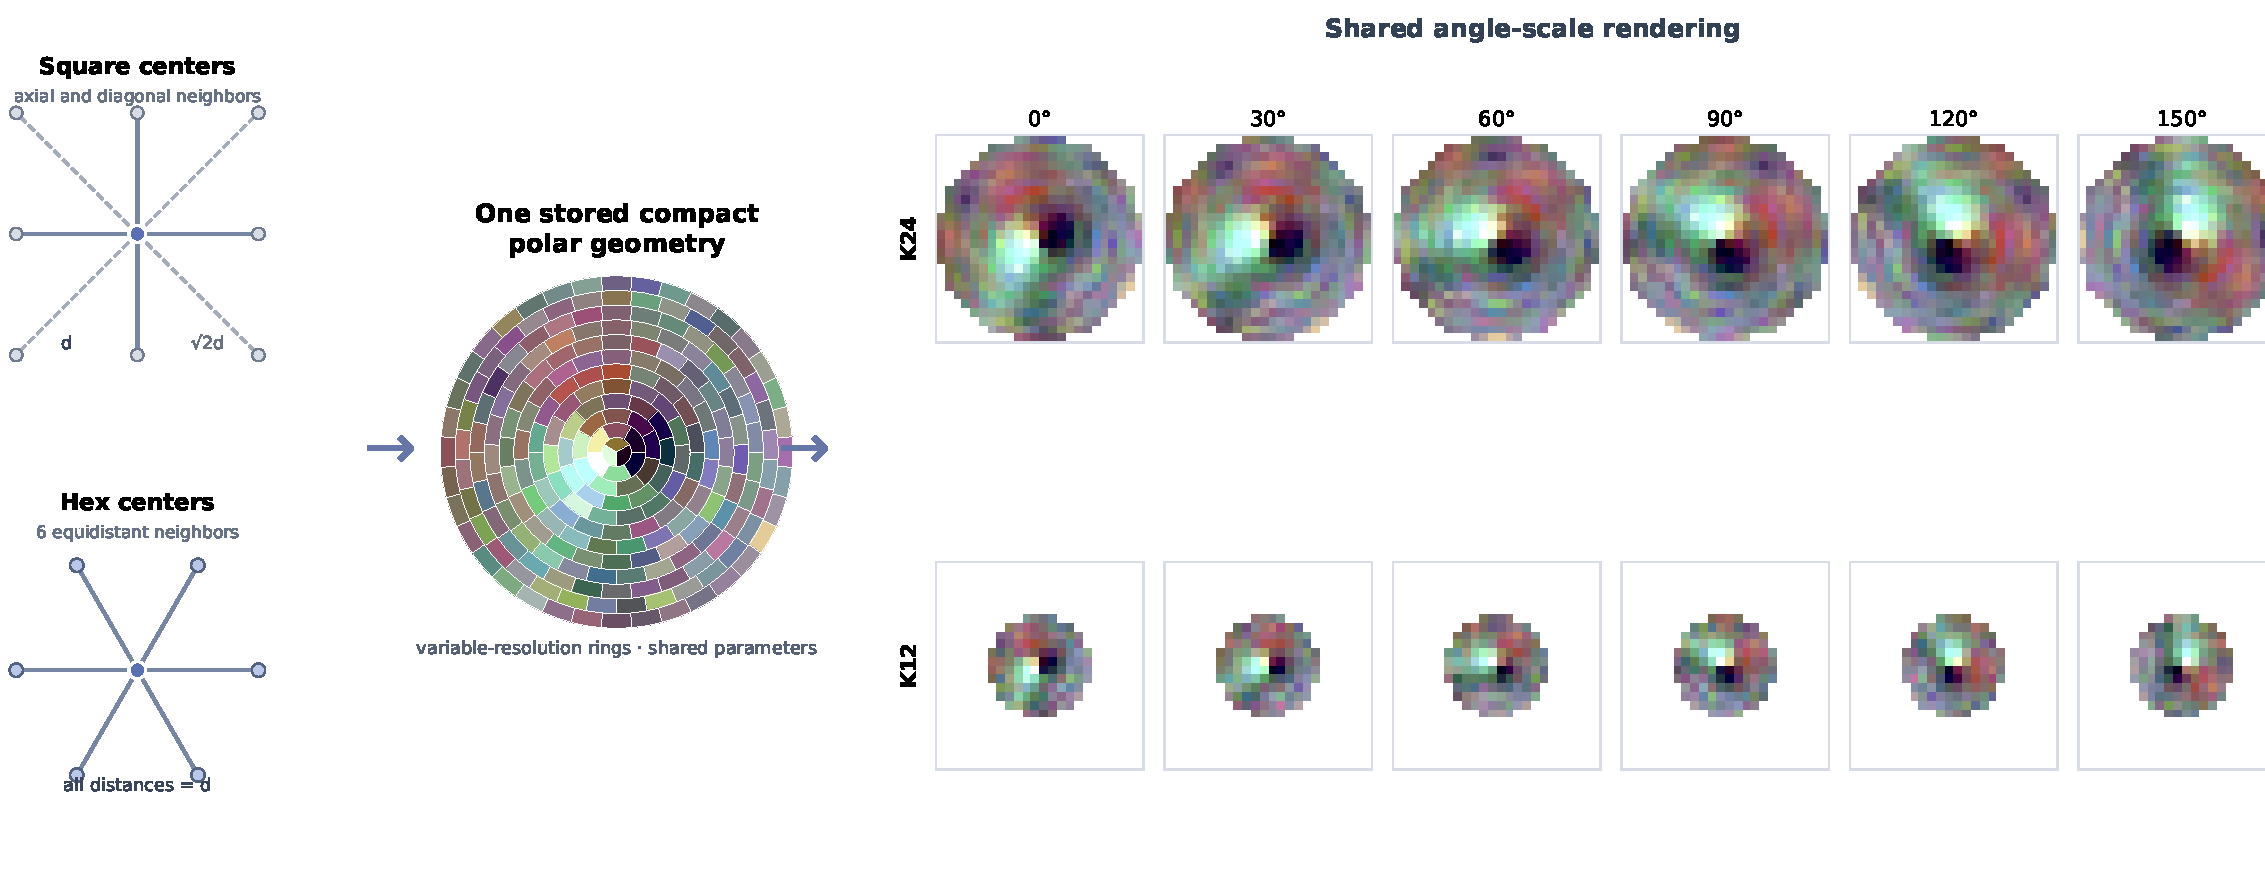
\includegraphics[width=1.10\textwidth]{figs/02_hex_multiscale_multiangle_kernels.pdf}}
  \caption{Hex-centered and shared angle--scale geometry. A compact
  variable-resolution polar prototype is rendered at two support sizes and six
  half-turn poses. The displayed kernels come from a trained model; the figure
  illustrates parameter sharing rather than an equivariance proof.}
  \label{fig:kernels}
\end{figure}

\subsection{Variable-resolution polar prototypes}

The tokenizer contains $P=96$ learned prototypes. Each prototype is stored in
polar coordinates over $R=12$ rings. We denote a half-turn geometry allocation
by \geom{D}{q}, where $D$ is the number of tested poses and $q$ is the base
number of angular samples added per radius. Under \geom{D}{q}, ring $r$ stores
$N_r=q(r+1)$ samples and pose $d$ uses $\theta_d=\pi d/D$, for
$r=0,\ldots,R-1$ and $d=0,\ldots,D-1$. The tested poses therefore uniformly
cover one half turn. Inner rings avoid angular parameters that cannot be
spatially resolved, while outer rings retain more detail. Bilinear
polar-to-Cartesian interpolation renders each prototype at a requested scale
and pose (Fig.~\ref{fig:kernels}).

For token $n$, prototype $p$, scale $k$, and tested direction $d$, the raw
matching score is the covered dot product
\begin{equation}
 s_{npkd}^{\geom{D}{q}}=\sum_{u\in\Omega_k}\gamma_k c_k(u)
 x_{n,k}(u)^\top w_{p,k,d}^{\geom{D}{q}}(u).
 \label{eq:match}
\end{equation}
No division by $\lVert x\rVert\lVert w\rVert$ is applied: this is a
dot-product kernel, not cosine similarity. Scores from both supports are
accumulated before routing, $s_{npd}=\sum_k s_{npkd}$.

The two evaluated allocations are \geom{4}{4}, which tests four poses at
$45^\circ$ increments, and \geom{6}{3}, which tests six poses at $30^\circ$
increments. The corresponding full directional periods used by the \look{}
fields contain $D_{\mathrm{global}}=2D$, hence eight and twelve bins. Direction
count and stored ring density therefore change together; the current experiment
compares these complete allocations and does not identify either factor in
isolation.

\subsection{Null-softmax circular-moment projection}

A learned scalar $s_p^{\varnothing}$ is appended to the direction logits of
each prototype. Let $\mathbf p_{np}$ contain the resulting pose probabilities
and the null probability:
\begin{equation}
 \mathbf p_{np}=\operatorname{softmax}(
 [s_{np0},\ldots,s_{np,D-1},s_p^{\varnothing}]).
 \label{eq:null}
\end{equation}
The null branch contributes zero, and the remaining direction probabilities
are not renormalized. A prototype can therefore lower its total activation
when none of the tested poses is appropriate.

Using the angles defined by \geom{D}{q}, each prototype emits its first
circular moment,
\begin{equation}
 z_{np}=\sum_{d=0}^{D-1}p_{npd}
 \begin{bmatrix}\cos\theta_d&\sin\theta_d\end{bmatrix}^{\!\top}.
 \label{eq:harmonic}
\end{equation}
Concatenating $z_{np}$ over 96 prototypes gives a 192-D token. This shares the
output basis across directions instead of learning a separate 192-D value
vector for every pose.

\subsection{Image-conditioned \look{} bias}
\label{sec:image-look}

Image \look{} uses one raw-image probe for each of the $12\times3=36$
layer--head pairs. Image-to-ring extraction does not record image gradients,
whereas probe and field parameters remain learnable. A probe returns
null-softmax pose weights $\pi_{bqhkd}$ for batch item $b$, query token $q$,
head $h$, scale $k$, and direction $d$.

Each head stores a signed canonical field
$G_h\in\R^{R_L\times D_L}$. Here $R_L=2|\mathcal K|=4$, and $D_L=2D$ follows
the tokenizer period: eight bins for \geom{4}{4} and twelve for \geom{6}{3}. Rotating and
radially interpolating $G_h$ yields a field $F_{hkdqj}$ over key token $j$.
The attention bias is
\begin{equation}
 B_{bhqj}^{\mathrm{img}}=\sum_{k,d}\pi_{bqhkd}F_{hkdqj}.
 \label{eq:image-look}
\end{equation}
The null route contributes zero. Since the field is conditioned on the query
token's local evidence, generally $B_{bhqj}\neq B_{bhjq}$.

\subsection{Token-conditioned Feature \look{}}
\label{sec:center-look}

Feature \look{} removes the raw-image probe and operates directly on the 96
cosine/sine pairs of each tokenizer output before adding positional embeddings.
The tokenizer output bias is subtracted first. The pairs are divided evenly
across three heads, giving 32 pairs per head. A probe group $g$ learns six axis
detectors $A_{ghapc}$ and computes
\begin{equation}
 a_{bngha}=\sum_{p,c}\bar z_{bnhpc}A_{ghapc}+\beta_{gha},
 \label{eq:center-probe}
\end{equation}
where $a\in\{1,\ldots,6\}$ indexes half-turn axes and $\bar z$ denotes the
bias-corrected tokenizer output. Appending a learned null score and applying
softmax produces pose weights.

Every one of the first 11 Transformer blocks and its three heads retains an
independent $4\times12$ field. A single pose probe may be reused by $G$
consecutive blocks, requiring $\lceil11/G\rceil$ groups. This separates the
cost of recognizing token pose from the layer-specific choice of where to
look. Feature \look{} is omitted from the final block because patch-to-patch
bias there cannot affect that same block's CLS output. If Image and Feature
\look{} are enabled together, their bases can be concatenated because the
structured additive attention construction is linear.

\subsection{Transformer backbone}

All ViT variants use a DeiT-Tiny-sized backbone with embedding dimension 192,
12 blocks, three attention heads, MLP ratio 4, and a CLS classifier. Absolute
positional embeddings are either enabled or disabled as an explicit ablation.
The large compact matching operations use mixed precision, while the small
routing softmax is evaluated in FP32.

\section{Experiments}

\subsection{Dataset and training protocol}

We use ImageNet-100 with 100 classes, 130,000 training images, and 5,000
validation images. All main-table models are trained from scratch for 20
epochs at $224\times224$ resolution with no pretrained weights or teacher.
Training uses two NVIDIA T4 GPUs, batch size 256 per GPU (global batch 512),
AdamW, initial learning rate $5\times10^{-4}$, minimum learning rate
$10^{-6}$, weight decay 0.05, two warmup epochs, cosine decay, label smoothing
0.1, gradient clipping at 1.0, mixed precision, and seed 0.

The training transform comprises random resized crop with bicubic
interpolation, horizontal flip, RandAugment with two operations and magnitude
9, ImageNet normalization, and random erasing with probability 0.25.
Validation resizes to 256, center-crops to 224, and applies ImageNet
normalization. We report the best validation top-1 and the top-5 from the same
epoch. Only one seed is complete, so the study is a controlled architectural
ablation rather than a statistically conclusive benchmark.

\subsection{Compared configurations}

\textbf{Standard} is the ordinary square $16\times16$ DeiT patch projection.
\textbf{Hex only} changes patch centers and support without rotating
prototypes. \textbf{Hex \geom{4}{4}} and \textbf{Hex \geom{6}{3}} use the two
allocations defined in Sec.~3.3: in \geom{D}{q}, $D$ counts tested half-turn
poses and $q$ gives the per-radius base sampling factor. For each rotating
tokenizer, we compare PE only, Image \look{} only, and PE+Image \look{}. We
then fix Hex \geom{6}{3} and PE and vary the Feature \look{} sharing span $G$.

The main comparison additionally includes three rotation-aware controls.
\textbf{Equi-ViT/GMR} adapts the published Gaussian-mixture-ring operator
\citep{chen2026equivit} to the common DeiT-sized classifier,
\textbf{ARC Adaptive} predicts bounded input-conditioned rotations for a bank
of patch kernels \citep{pu2023arc}, and \textbf{GE-ViT p4 local} preserves a
four-state orientation axis through a local group-attention backbone
\citep{xu2023e2vit}. These are operator-level adaptations under the
shared ImageNet-100 recipe, not claims to reproduce the original papers' full
datasets and training systems.

Parameter counts come from stored model summaries. Cross-version wall times are
omitted because shared Kaggle sessions do not support controlled hardware
comparisons.

\clearpage
\section{Results}
\subsection{Main comparison and local rotation response}
\begin{center}
\centering
\captionof{table}{Local re-evaluation of the six saved checkpoints. The $0^\circ$
columns evaluate the unrotated 5,000-image ImageNet-100 validation set. Local
means average the 12 nonzero rotations from $-30^\circ$ to $+30^\circ$ in
$5^\circ$ increments. JSD is the mean Jensen--Shannon divergence from each
model's own $0^\circ$ predictive distribution and is confidence-sensitive.}
\label{tab:main}
\small
\setlength{\tabcolsep}{6.0pt}
\begin{tabular}{lrrrrrr}
\toprule
& \multicolumn{2}{c}{$0^\circ$ validation} &
  \multicolumn{3}{c}{Local rotations} & \\
\cmidrule(lr){2-3}\cmidrule(lr){4-6}
Model & Top-1 & Top-5 & Mean Top-1 & Mean Top-5 & $100\!\times$ Mean JSD $\downarrow$ & Params (M)\\
\midrule
Standard DeiT-Tiny              & 51.54 & 79.12 & 49.91 & 77.45 & \third{5.27} & 5.544\\
SHARE \geom{4}{4} + Image \look{}  & \third{53.68} & \third{80.46} & \third{51.25} & \third{78.89} & 5.65 & 5.501\\
SHARE \geom{6}{3} + dual \look{}   & \underline{55.52} & \underline{81.80} & \underline{52.82} & \textbf{79.98} & 5.64 & 5.497\\
Equi-ViT / GMR                  & 41.52 & 70.40 & 41.08 & 70.12 & \textbf{3.22} & 5.424\\
ARC Adaptive                    & 49.38 & 76.56 & 47.76 & 75.70 & \underline{5.25} & 5.986\\
GE-ViT p4 local                 & \textbf{56.06} & \textbf{82.04} & \textbf{52.94} & \underline{79.45} & 5.88 & 5.509\\
\bottomrule
\end{tabular}
\end{center}

For predictive distributions $p_{i,\theta}$ and $p_{i,0}$, let
$m_{i,\theta}=\tfrac12(p_{i,\theta}+p_{i,0})$. We report
\begin{equation}
\overline{\mathrm{JSD}}_{100}
=\frac{100}{12N}\sum_{\theta\in\{\pm5^\circ,\ldots,\pm30^\circ\}}
\sum_{i=1}^{N}\left[
\tfrac12 D_{\mathrm{KL}}(p_{i,\theta}\Vert m_{i,\theta})+
\tfrac12 D_{\mathrm{KL}}(p_{i,0}\Vert m_{i,\theta})\right].
\label{eq:rotation-jsd}
\end{equation}
Bold, underlined, and blue values denote the best, second-best, and third-best
result in each evaluation column, respectively.

Table~\ref{tab:main} separates ordinary validation accuracy from local
rotation behavior. SHARE \geom{6}{3} is within 0.12 top-1 points of GE-ViT after
averaging the local rotations and has the highest mean top-5, while retaining
fewer parameters than Standard. Relative to Standard, its local means improve
by 2.91 top-1 and 2.53 top-5 points. GE-ViT has the strongest unrotated and
mean local top-1 results, consistent with retaining an explicit orientation
axis throughout its backbone. ARC Adaptive is below Standard under this short
from-scratch recipe. Equi-ViT/GMR has the smallest JSD but also much lower
accuracy; its small probability drift must therefore not be read as superior
classification robustness in isolation.

\begin{center}
  \centering
  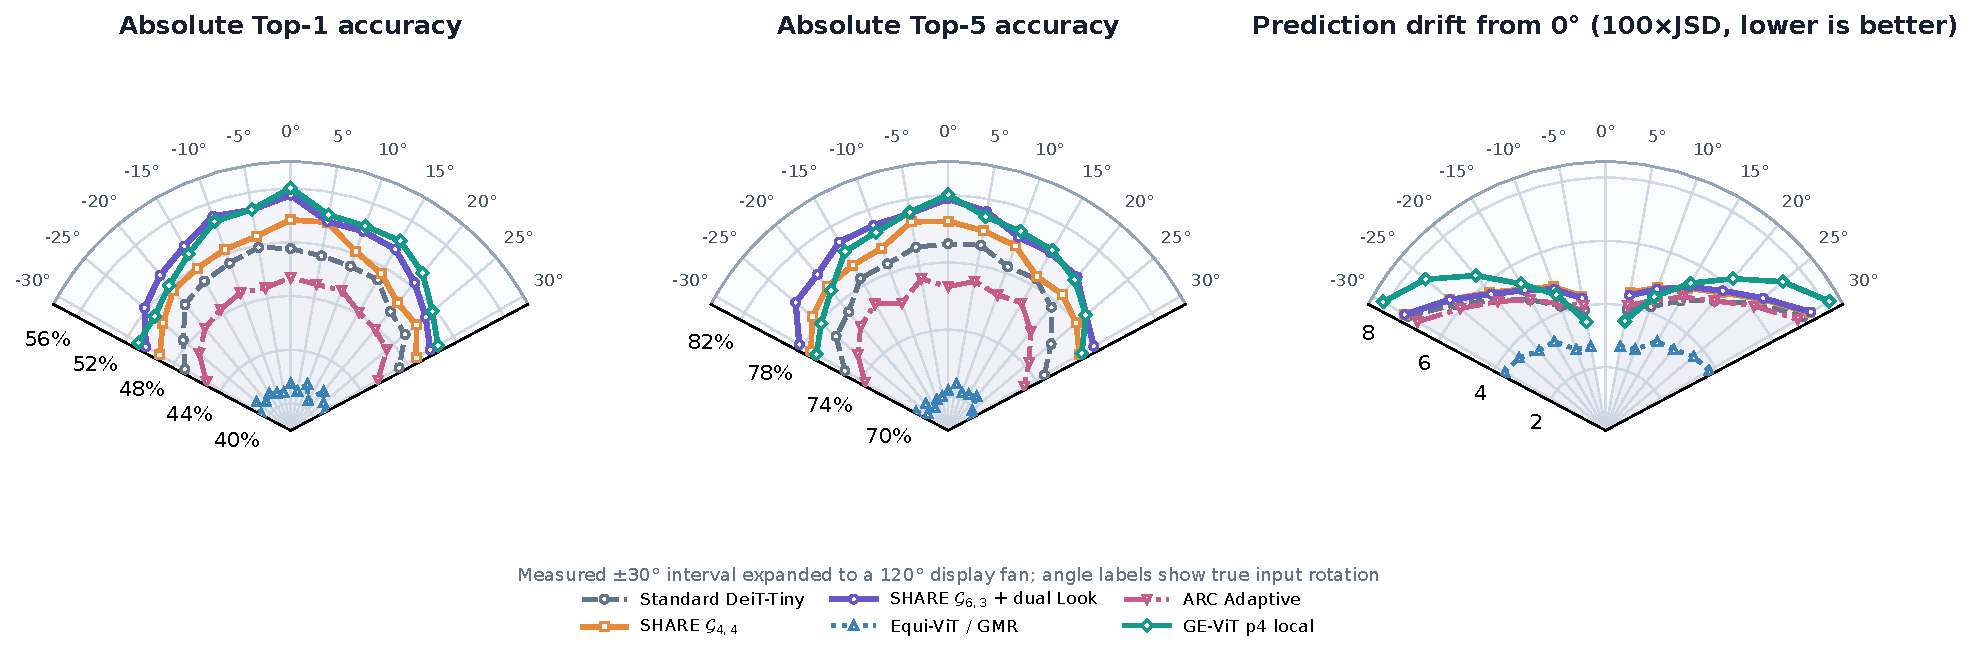
\includegraphics[width=\textwidth]{figs/08_all5000_six_models_rotation_fans.pdf}
  \captionof{figure}{Local rotation response on all 5,000 ImageNet-100 validation
  images. Left and middle show absolute top-1 and top-5 accuracy. Right shows
  $100\times$ Jensen--Shannon drift from each model's own $0^\circ$ distribution; the
  tautological zero-angle JSD point is omitted, leaving the positive and
  negative branches visually separate. The measured $\pm30^\circ$ range is
  expanded to a $120^\circ$ display fan while labels retain the true input
  angles. Every model receives identical bilinearly rotated inputs.}
  \label{fig:local-rotation-fans}
\end{center}

Figure~\ref{fig:local-rotation-fans} exposes three complementary effects.
First, top-1 declines smoothly with increasing absolute rotation for all
models, rather than failing at one isolated angle. Second, the top-5 panel
shows that SHARE \geom{6}{3} retains a stronger candidate-class set across the
local interval even where GE-ViT has slightly higher top-1. Third, JSD measures
probability movement that top-$k$ accuracy cannot expose. Equi-ViT/GMR's low
JSD accompanies low confidence and low accuracy, whereas GE-ViT's larger JSD
coexists with the strongest top-1; the three panels must therefore be read
together. SHARE \geom{6}{3} also shows a small sign asymmetry: positive rotations
average 0.77 top-1 points below matched negative rotations. Because Standard,
ARC, Equi-ViT/GMR, and GE-ViT do not share this sign, we treat it as a
model-specific diagnostic of the half-angle/\look{} pathway, not as evidence
of a universal preprocessing bias or exact equivariance.

\subsection{Tokenizer and Image \look{} ablation}

\begin{table}[t]
\centering
\caption{Tokenizer geometry and positional-signal ablation under the aligned
20-epoch ImageNet-100 recipe. Geometry symbols follow Sec.~3.3.
$\Delta$ is the percentage-point change
from Standard. Top-5 is taken at the best-top-1 epoch.}
\label{tab:tokenizer}
\small
\setlength{\tabcolsep}{5.1pt}
\begin{tabular}{lccrrrrr}
\toprule
Tokenizer & PE & Image \look{} & Top-1 & $\Delta$Top-1 & Top-5 & $\Delta$Top-5 & Params (M)\\
\midrule
Standard & \yes & \no & 51.52 & -- & 79.12 & -- & 5.544\\
Hex only & \yes & \no & 51.30 & $-0.22$ & 79.14 & $+0.02$ & 5.597\\
Hex \geom{4}{4} & \yes & \no & 53.56 & $+2.04$ & 80.40 & $+1.28$ & 5.486\\
Hex \geom{4}{4} & \no & \yes & 50.26 & $-1.26$ & 77.72 & $-1.40$ & 5.463\\
Hex \geom{4}{4} & \yes & \yes & 53.70 & $+2.18$ & 80.46 & $+1.34$ & 5.501\\
Hex \geom{6}{3} & \yes & \no & 54.54 & $+3.02$ & 80.46 & $+1.34$ & 5.464\\
Hex \geom{6}{3} & \no & \yes & 52.42 & $+0.90$ & 79.48 & $+0.36$ & 5.453\\
\textbf{Hex \geom{6}{3}} & \yes & \yes & \textbf{55.04} & \textbf{$+3.52$} & \textbf{81.80} & \textbf{$+2.68$} & 5.491\\
\bottomrule
\end{tabular}
\end{table}

\paragraph{Directions versus ring resolution.}
The \geom{4}{4} configuration evaluates four poses over a half turn and uses
$q=4$; \geom{6}{3} evaluates six poses while using $q=3$. Thus pose count and
polar storage density move in opposite
directions in this experiment. They are a coupled geometry choice rather than
an isolated direction-count ablation.

Table~\ref{tab:tokenizer} shows that the plain Hex tokenizer does not improve
top-1, indicating that a staggered lattice alone is insufficient. Rotating
prototype matching is the main source of gain: PE-only \geom{4}{4} and
\geom{6}{3} improve over Standard by 2.04 and 3.02 points, respectively.
\geom{6}{3} outperforms \geom{4}{4} under all three positional configurations.
Because this comparison
jointly changes the number of tested directions and samples stored per ring, it
supports the complete six-direction allocation, not a claim about either
factor in isolation.

Image \look{} does not replace absolute location: Look-only trails PE+Look in
both geometry settings. It is nevertheless complementary to PE. For \geom{6}{3},
adding Image \look{} increases top-1 from 54.54 to 55.04 and top-5 from 80.46
to 81.80. The best model exceeds Standard by 3.52 top-1 and 2.68 top-5 points
while using 5.491M instead of 5.544M parameters. The gain is therefore not
explained by a larger parameter budget.

\subsection{Feature \look{} sharing span}

Figure~\ref{fig:center-sharing} reveals a non-monotonic sharing trade-off. Recomputing a
distinct pose detector for every block ($G=1$) is not best. Moderate sharing
with $G=3$ or $4$ improves top-1, and $G=4$ reaches 55.18\%, slightly above the
55.04\% Image \look{} model. More aggressive sharing ($G=6$ or $12$) falls
back to approximately 54.5\%. This is consistent with a pose cue that is
reusable across nearby layers but too coarse when globalized across the
network. Since all rows use one seed and differences are small, this remains a
bounded interpretation rather than a statistical conclusion.

The optimum changes when Image \look{} is also active. As shown in
Fig.~\ref{fig:center-sharing}, the dual-\look{} model peaks at $G=3$ with
55.54\% top-1, 0.50 points above PE+Image \look{} and 0.54 points above the
PE+Feature \look{} model at the same span. The older dual-\look{} $G=4$ point
used the pre-optimization expanded kernel, so it is retained for provenance
rather than treated as a controlled kernel-speed comparison. Together, the
curves support an interaction between branch placement and sharing span rather
than unconditional additivity or redundancy.

\begin{figure}[t]
  \centering
  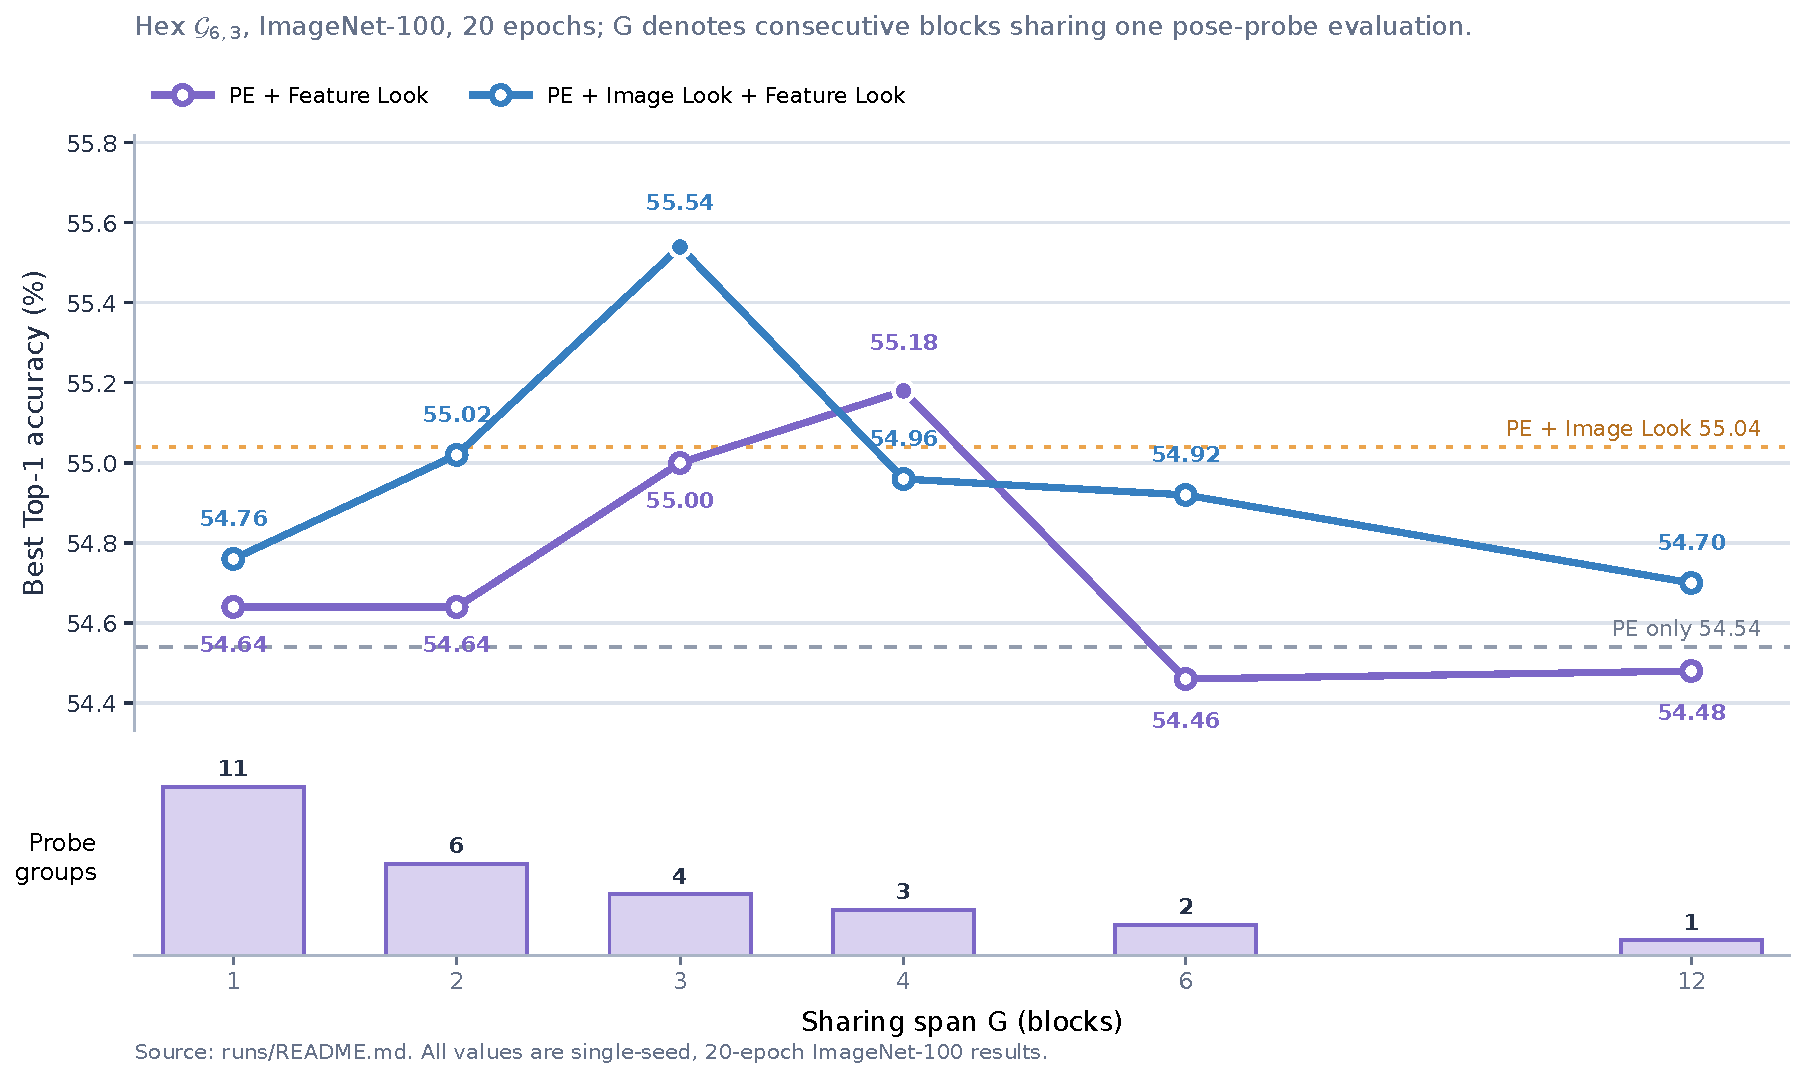
\includegraphics[width=0.94\textwidth]{figs/05_feature_look_sharing_span.pdf}
  \caption{Feature \look{} probe-sharing ablation. Purple uses PE+Feature
  \look{}; blue additionally enables Image \look{}. The lower panel reports
  the architectural number of probe evaluations. All values are single-seed
  20-epoch results.}
  \label{fig:center-sharing}
\end{figure}

The lower panel reports the architectural number of pose-probe evaluations;
wall-clock time is omitted because cross-version timing was not controlled.
Each block still retains its own $4\times12$ output field.

\subsection{Learned directed fields}

\begin{figure}[t]
  \centering
  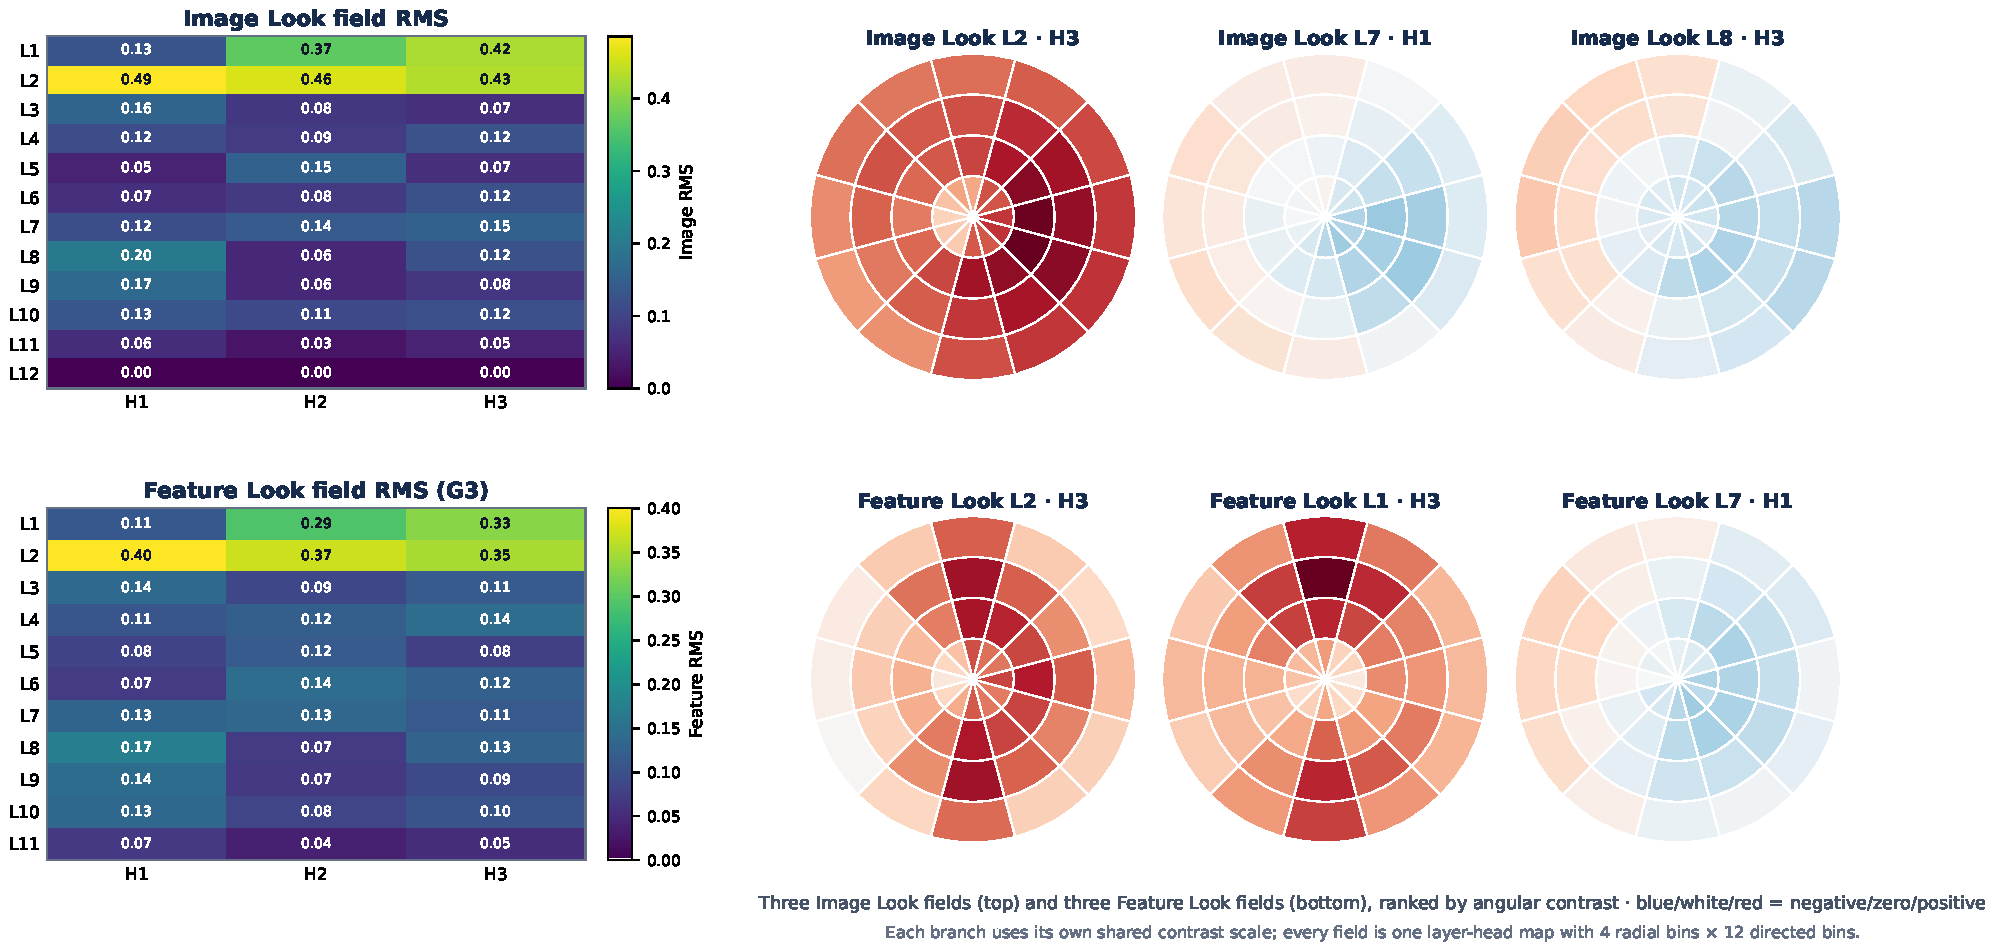
\includegraphics[width=0.93\textwidth]{figs/03_half6d3r_look_bias_fields.pdf}
  \caption{Learned parameters from the best dual-\look{} model (\geom{6}{3} + PE
  + Image \look{} + G3 Feature \look{}). Left: per-layer, per-head RMS
  magnitude for Image and Feature \look{}, shown with separate color scales.
  Right: the three layer--head fields with the largest angular contrast from
  each branch, measured after removing the mean of every radial ring. Each
  signed $4\times12$ map is shown separately rather than mixing heads as RGB.
  G3 reuses one pose probe for each consecutive three-layer group, while every
  active layer retains its own output field. Nonuniform fields are an
  implementation-level observation, not a causal interpretability claim.}
  \label{fig:look-fields}
\end{figure}

Figure~\ref{fig:look-fields} shows that the learned fields are neither uniform
across heads nor constant across depth. This visualization verifies variation
in the implemented directed fields, but it does not establish semantic part
discovery, causal explanation, or exact rotation behavior.

\section{Discussion}

\subsection{What the ablations establish}

Within the aligned setup, three conclusions are supported. First, changing the
sampling lattice alone is insufficient; learned multi-pose prototype matching
is the important tokenizer change. Second, absolute PE and Image \look{} are
complementary: the former supplies persistent token identity, while the latter
adds image-conditioned directed relations. Third, Feature \look{} can reuse one
pose detector over a short layer span without sharing the layer-specific
attention field, but global probe sharing loses accuracy. Its best span also
depends on placement: G4 is best with PE alone, whereas G3 is best when Image
\look{} is active, where the two directed branches provide the strongest
observed result.

The six-direction allocation is consistently better than the four-direction
allocation in the tested configurations. It also uses a more compact angular
storage per radius, so the present experiment cannot attribute the gain only
to direction count. This coupling is an explicit target for a future factorial
ablation.

\subsection{Limitations}

The current evidence has five important limits. (1) Only one random seed is
complete, so differences of a few tenths of a point may reflect training
variance. (2) The 20-epoch schedule is short and may rank architectures
differently from a converged recipe. (3) The method samples a finite set of
rotations; interpolation, image boundaries, and the unconstrained backbone
prevent a claim of exact equivariance. (4) Evaluation covers one classification
dataset and does not establish ImageNet-1K, detection, segmentation,
robustness, or transfer gains. (5) shared Kaggle wall times are insufficient
for a hardware-efficiency claim.

The visualizations expose how the implemented routing behaves, but the learned
fields are operational model components rather than causal explanations of a
prediction. Their semantic interpretation must remain descriptive.

\subsection{Next validation}

The highest-priority experiment is an angle--scale controlled benchmark that
trains on one set of poses and evaluates on interleaved unseen poses. This would
directly test whether shared prototypes improve interpolation. A factorial
tokenizer experiment should independently vary tested direction count and ring
storage density. Multi-seed ImageNet-100 runs under a longer schedule are
needed for confidence intervals. Longer ImageNet-100 training and ImageNet-1K
evaluation would then test whether the observed gains persist beyond the
current short, single-dataset setting.

\section{Conclusion}

We presented \method{}, a geometric interface between images and global
self-attention. Hex-centered multi-scale patches are matched against rotating
variable-resolution polar prototypes and compressed through null-softmax
circular moments. Image \look{} converts independent raw-image evidence into
directed attention fields, while Feature \look{} obtains a lighter pose probe
directly from token coordinates and exposes a useful local layer-sharing
scale. In the current aligned ImageNet-100 study, the six-direction Image
\look{} model improves top-1 from 51.52\% to 55.04\%; Feature \look{} with PE
reaches 55.18\%; and their best observed combination reaches 55.54\% at G3,
without increasing the baseline parameter count. The results motivate explicit
local pose and scale as complements to positional encoding, while leaving exact
equivariance, statistical confirmation, and broader task generalization open.

\raggedbottom
\footnotesize
\bibliographystyle{plainnat}
\bibliography{references}

\end{document}
